\chapter{particular presets} 
\label{sec:presets}
\lstset{style=6502Style}
\lstset{ 
   aboveskip=5pt,
   belowskip=0pt,
}

\begin{definition}[Jeffrey Says]
\setlength{\intextsep}{0pt}%
\setlength{\columnsep}{3pt}%
\begin{wrapfigure}{l}{0.12\textwidth}

\includegraphics[width=\linewidth]{src/callout/psych.png} 
\end{wrapfigure}
\small
SHIFT plus any of the top row of
preset keys: Stores all the parameters for later, instantaneous,
recall by pressing that preset key. Use to store your favourites for
recall instantly without fiddling with all the parameters. 16 presets
available.
\end{definition}

Psychedelia allows you to save whatever your configuration is at the moment for easy use later on.
The 16 available slots come pre-configured with some colorful configurations. We'll take a look at them
all here, as well as understanding how the presets are loaded by the player.

On the following two page we show the first preset configuration in action and on the facing page the 
data structure that sits behind it, enumerating all the settings a 'preset' contains. Elsewhere in this
chapter we illustrate the 15 other presets slightly more concisely, with a diagram and a briefer version
of the same data structure.

\clearpage                                                                 
\begin{figure}[H]                                                          
  \centering                                                             
  \begin{adjustbox}{width=14cm,center}                                   
  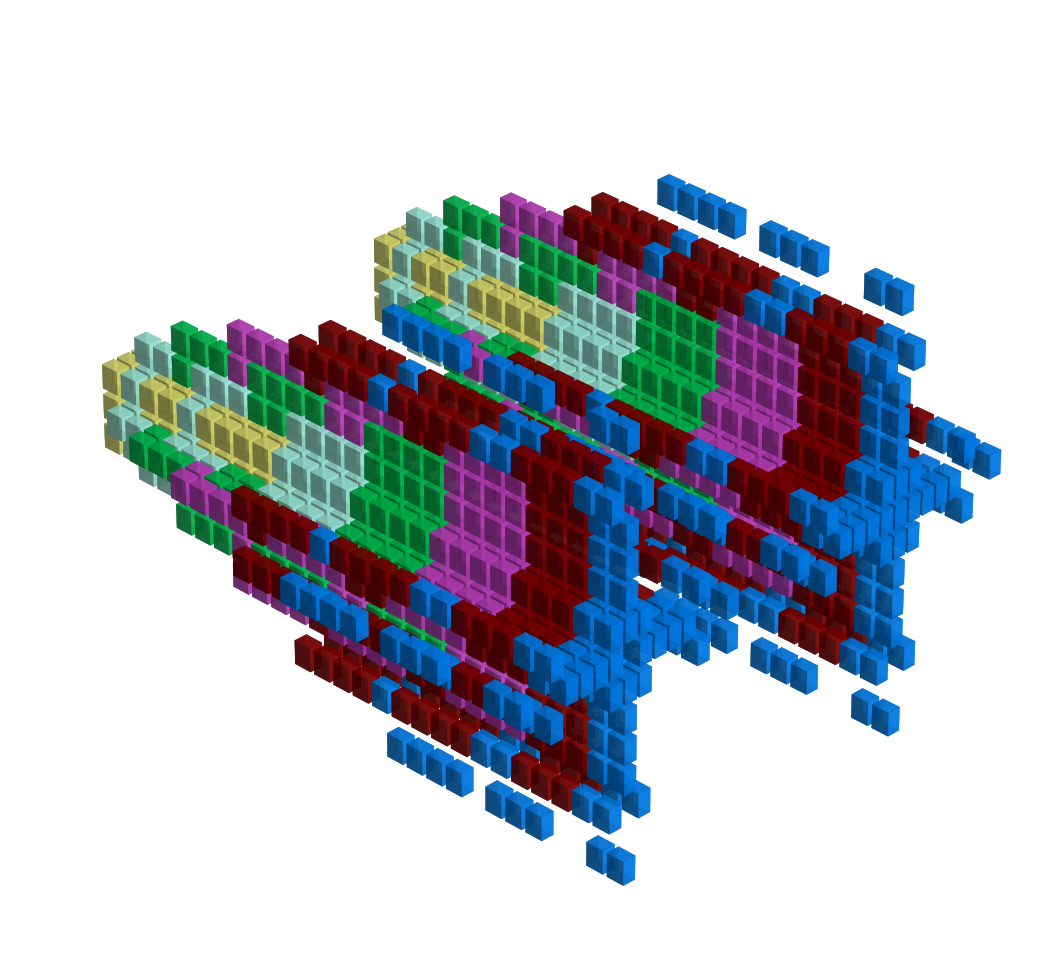
\includegraphics[width=14cm]{src/presets/pattern0-45.png}%           
  \end{adjustbox}                                                        
\caption{Evolution of Preset 0.}                                           
\end{figure}                                                               
\clearpage                                                                 
                                                                           
\begin{lstlisting}[basicstyle=\ttfamily\scriptsize,caption=Data structure for Preset 0.]
;preset0
  ; unusedPresetByte: Unused Byte
  .BYTE $00
  ; smoothingDelay: 'Because of the time taken to draw larger patterns speed
  ; increase/decrease is not linear. You can adjust the 'compensating delay'
  ; which often smooths out jerky patterns. Can be used just for special FX),
  ; though. Suck it and see.'
  .BYTE $0C
  ; cursorSpeed: 'Gives you a slow or fast little cursor, according to setting.'
  .BYTE $02
  ; bufferLength: 'Larger patterns flow more smoothly with a shorter
  ; Buffer Length - not so many positions are retained so less plotting to do.
  ; Small patterns with a long Buffer Length are good for 'steamer' effects.
  ; N.B. Cannot be adjusted whilst patterns are actually onscreen.'
  .BYTE $1F
  ; pulseSpeed: 'Usually if you hold down the button you get a continuous
  ; stream. Setting the Pulse Speed allows you to generate a pulsed stream, as
  ; if you were rapidly pressing and releasing the FIRE button.'
  .BYTE $01
  ; indexForColorBarDisplay: 'The initial index for the color displayed
  ; in the color bar when adjusting the colors for each step.'
  .BYTE $01
  ; lineWidth: 'Sets the width of the lines produced in Line Mode.'
  .BYTE $07
  ; sequencerSpeed: 'Controls the rate at which sequencer feeds in its data. '
  .BYTE $04
  ; pulseWidth: 'Sets the length of the pulses in a pulsed stream output.
  ; Don't worry about what that means - just get in there and mess with it.'
  .BYTE $01
  ; baseLevel: 'Controls how many 'levels' of pattern are plotted.'
  .BYTE $07
  ; presetColorValuesArray: 'Allows you to set the colour for each of the
  ; seven pattern steps. Set up the colour you want, press RETURN, and the
  ; command offers the next colour along, up to no. 7, then ends. Cannot be
  ; adjusted while patterns being generated.'
  .BYTE BLACK,BLUE,RED,PURPLE,GREEN,CYAN,YELLOW,WHITE
  ; trackingActivated: 'Controls whether logic-seeking is used in the
  ; buffer or not. The upshot of this for you is a slightly different feel -
  ; continuous but fragmented when ON, or together-ish bursts when OFF. Try it.'
  .BYTE $00
  ; lineModeActivated: 'A bit like drawing with the Aurora Borealis'
  .BYTE $00
  ; presetIndex: 'This calls in one of the 16 presets, stored Lightsynth
  ; parameters which give different effects. Try them all out io see some uf
  ; the multitude of effects which you cai achieve using the system. Some are
  ; fast, some slow, some pulse, others swirl. Play with them all, try them to
  ; different music.'
  .BYTE $00
  ; currentPatternElement: 'Initial pattern used by this preset.'
  .BYTE $00
  ; currentSymmetrySetting: 'Current symmetry setting.'
  ; Possible values are 0 - 4:
  ; 'NO SYMMETRY     '
  ; 'Y-AXIS SYMMETRY '
  ; 'X-Y SYMMETRY    '
  ; 'X-AXIS SYMMETRY '
  ; 'QUAD SYMMETRY   '
  .BYTE $01
  ; Unused Data.
  .BYTE $FF,$00,$FF,$FF,$00,$FF,$00,$FF,$00
\end{lstlisting}

\clearpage
\begin{minipage}[b]{0.48\linewidth}
\begin{figure}[H]                                                          
  \centering                                                             
  \begin{adjustbox}{width=7cm,center}                                   
  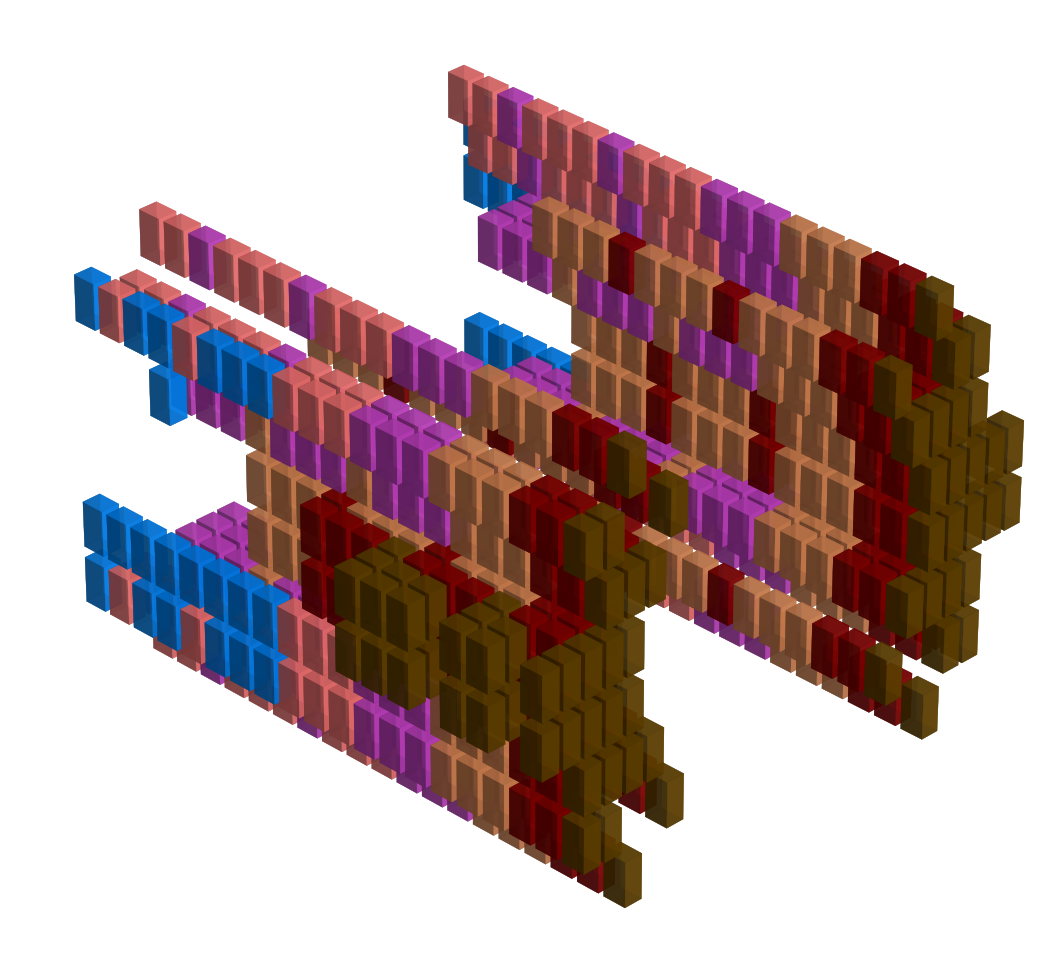
\includegraphics[width=7cm]{src/presets/pattern1-45.png}%           
  \end{adjustbox}                                                        
\caption{Evolution of Preset 1.}                                           
\end{figure}                                                               
\end{minipage}
\hspace{0.1cm}
\begin{minipage}[b]{0.48\linewidth}                            
                                                                           
\begin{lstlisting}[basicstyle=\ttfamily\scriptsize,caption=Data structure for Preset 1.]
preset1
  .BYTE $00 ; unusedPresetByte
  .BYTE $0C ; smoothingDelay
  .BYTE $02 ; cursorSpeed
  .BYTE $28 ; bufferLength
  .BYTE $01 ; pulseSpeed
  .BYTE $0E ; indexForColorBarDisplay
  .BYTE $07 ; lineWidth
  .BYTE $08 ; sequencerSpeed
  .BYTE $01 ; pulseWidth
  .BYTE $07 ; baseLevel
  ; presetColorValuesArray: 
  .BYTE BLACK,BROWN,RED,ORANGE,PURPLE,LTRED,BLUE,LTBLUE
  .BYTE $FF ; trackingActivated
  .BYTE $00 ; lineModeActivated
  .BYTE $01 ; presetIndex
  .BYTE $01 ; currentPatternElement
  .BYTE $04 ; currentSymmetrySetting
\end{lstlisting}
\end{minipage}
\begin{minipage}[b]{0.48\linewidth}

\begin{figure}[H]                                                          
  \centering                                                             
  \begin{adjustbox}{width=7cm,center}                                   
  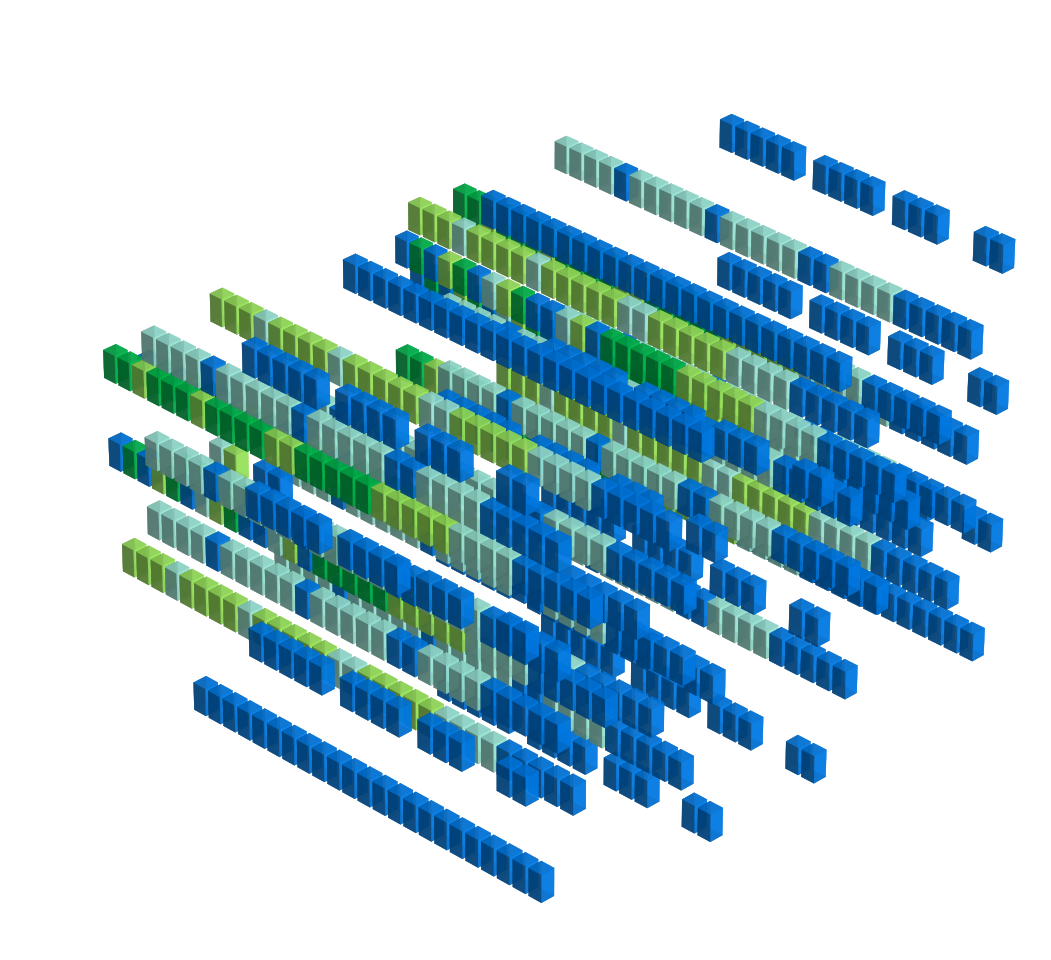
\includegraphics[width=7cm]{src/presets/pattern2-45.png}%           
  \end{adjustbox}                                                        
\caption{Evolution of Preset 2.}                                           
\end{figure}                                                               
\end{minipage}
\hspace{0.1cm}
\begin{minipage}[b]{0.48\linewidth}                            
                                                                           
\begin{lstlisting}[basicstyle=\ttfamily\scriptsize,caption=Data structure for Preset 2.]
preset2
  .BYTE $00 ; unusedPresetByte
  .BYTE $0B ; smoothingDelay
  .BYTE $02 ; cursorSpeed
  .BYTE $28 ; bufferLength
  .BYTE $01 ; pulseSpeed
  .BYTE $01 ; indexForColorBarDisplay
  .BYTE $07 ; lineWidth
  .BYTE $0B ; sequencerSpeed
  .BYTE $01 ; pulseWidth
  .BYTE $07 ; baseLevel
  ; presetColorValuesArray: 
  .BYTE BLACK,BLUE,LTBLUE,CYAN,LTGREEN,GREEN,LTBLUE,BLUE
  .BYTE $FF ; trackingActivated
  .BYTE $00 ; lineModeActivated
  .BYTE $05 ; presetIndex
  .BYTE $05 ; currentPatternElement
  .BYTE $01 ; currentSymmetrySetting
\end{lstlisting}
\end{minipage}


\clearpage
\begin{minipage}[b]{0.48\linewidth}

\begin{figure}[H]                                                          
  \centering                                                             
  \begin{adjustbox}{width=7cm,center}                                   
  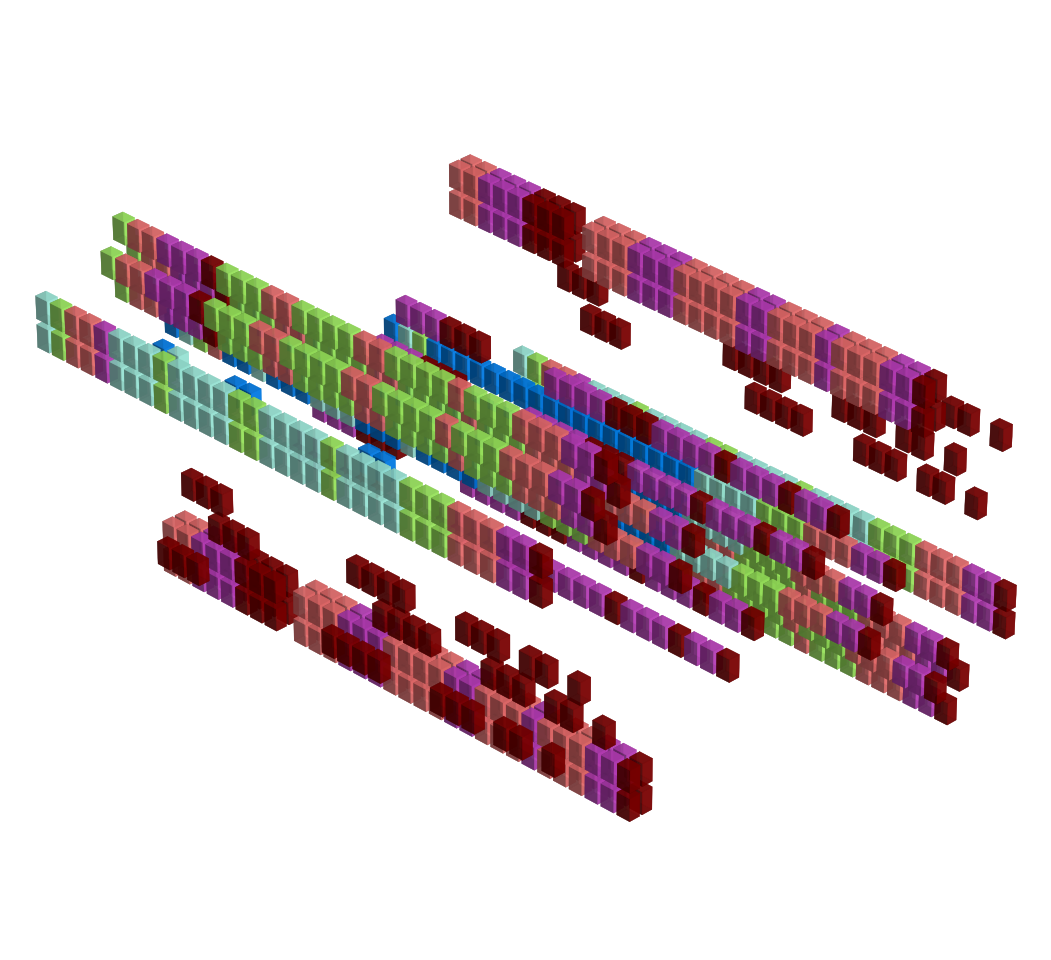
\includegraphics[width=7cm]{src/presets/pattern3-45.png}%           
  \end{adjustbox}                                                        
\caption{Evolution of Preset 3.}                                           
\end{figure}                                                               
\end{minipage}
\hspace{0.1cm}
\begin{minipage}[b]{0.48\linewidth}                            
                                                                           
\begin{lstlisting}[basicstyle=\ttfamily\scriptsize,caption=Data structure for Preset 3.]
preset3
  .BYTE $00 ; unusedPresetByte
  .BYTE $04 ; smoothingDelay
  .BYTE $02 ; cursorSpeed
  .BYTE $26 ; bufferLength
  .BYTE $01 ; pulseSpeed
  .BYTE $01 ; indexForColorBarDisplay
  .BYTE $07 ; lineWidth
  .BYTE $0A ; sequencerSpeed
  .BYTE $01 ; pulseWidth
  .BYTE $07 ; baseLevel
  ; presetColorValuesArray: 
  .BYTE BLACK,RED,PURPLE,LTRED,LTGREEN,CYAN,LTBLUE,BLUE
  .BYTE $00 ; trackingActivated
  .BYTE $00 ; lineModeActivated
  .BYTE $0E ; presetIndex
  .BYTE $0E ; currentPatternElement
  .BYTE $02 ; currentSymmetrySetting
\end{lstlisting}

\end{minipage}
\vspace*{-0.7cm}
\begin{minipage}[b]{0.48\linewidth}
\begin{figure}[H]                                                          
  \centering                                                             
  \begin{adjustbox}{width=7cm,center}                                   
  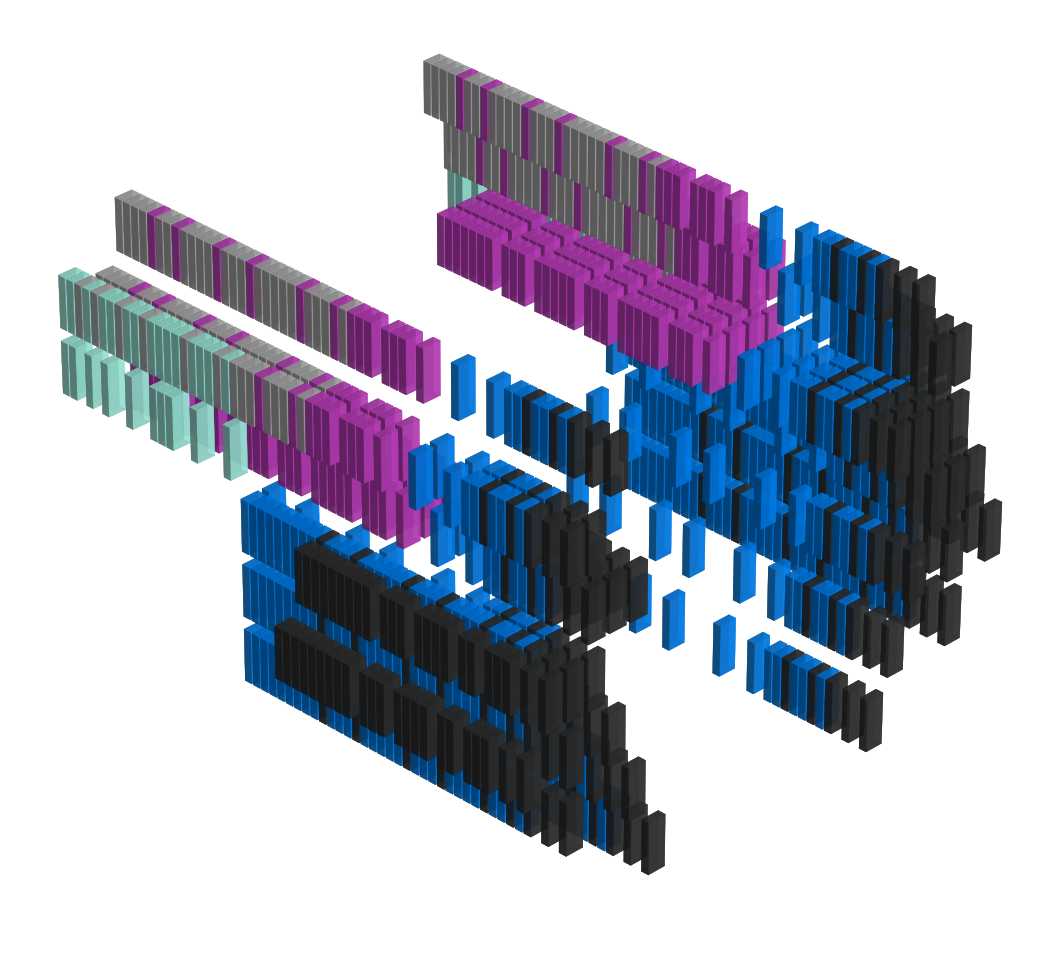
\includegraphics[width=7cm]{src/presets/pattern4-45.png}%           
  \end{adjustbox}                                                        
\caption{Evolution of Preset 4.}                                           
\end{figure}                                                               
\end{minipage}
\hspace{0.1cm}
\begin{minipage}[b]{0.48\linewidth}                            
                                                                           
\begin{lstlisting}[basicstyle=\ttfamily\scriptsize,caption=Data structure for Preset 4.]
preset4
  .BYTE $00 ; unusedPresetByte
  .BYTE $0C ; smoothingDelay
  .BYTE $01 ; cursorSpeed
  .BYTE $2B ; bufferLength
  .BYTE $01 ; pulseSpeed
  .BYTE $07 ; indexForColorBarDisplay
  .BYTE $07 ; lineWidth
  .BYTE $08 ; sequencerSpeed
  .BYTE $01 ; pulseWidth
  .BYTE $07 ; baseLevel
  ; presetColorValuesArray: 
  .BYTE BLACK,GRAY1,BLUE,GRAY2,PURPLE,GRAY3,CYAN,WHITE
  .BYTE $00 ; trackingActivated
  .BYTE $00 ; lineModeActivated
  .BYTE $01 ; presetIndex
  .BYTE $01 ; currentPatternElement
  .BYTE $01 ; currentSymmetrySetting
\end{lstlisting}
\end{minipage}
\clearpage

\clearpage
\textbf{Lines 1189-1231. \icode{\textbf{presetValueArray}}}
\begin{lstlisting}
; This is where the presets get loaded to. It represents
; the data structure for the presets.
; currentVariableMode is an index into this data structure
; when the user adjusts settings.
presetValueArray
unusedPresetByte        .BYTE $00
smoothingDelay          .BYTE $0C
cursorSpeed             .BYTE $02
bufferLength            .BYTE $1F
pulseSpeed              .BYTE $01
indexForColorBarDisplay .BYTE $01
lineWidth               .BYTE $07
sequencerSpeed          .BYTE $04
pulseWidth              .BYTE $01
baseLevel               .BYTE $07
presetColorValuesArray  .BYTE BLACK,BLUE,RED,PURPLE,GREEN,CYAN,YELLOW,WHITE
trackingActivated       .BYTE $FF
lineModeActivated       .BYTE $00
patternIndex            .BYTE $05
\end{lstlisting}

\textbf{Lines 1189-1231. \icode{\textbf{presetKeyCodes}}} 
\begin{lstlisting}
presetKeyCodes
        .BYTE KEY_LEFT,KEY_1,KEY_2,KEY_3,KEY_4,KEY_5,KEY_6,KEY_7
        .BYTE KEY_8,KEY_9,KEY_0,KEY_PLUS,KEY_MINUS,KEY_POUND
        .BYTE KEY_CLR_HOME,KEY_INST_DEL
\end{lstlisting}
\textbf{Lines 1189-1231. \icode{\textbf{CheckKeyboardInput}}} 
\begin{lstlisting}
;-------------------------------------------------------
; CheckKeyboardInput
;-------------------------------------------------------
CheckKeyboardInput   
        ...
        ; Check if one of the presets has been selected.
CheckIfPresetKeysPressed   

        LDX #$00
presetKeyLoop   
        CMP presetKeyCodes,X
        BEQ WriteTemplateTextForPreset
        INX 
        CPX #$10
        BNE presetKeyLoop

        JMP MaybeWPressed

WriteTemplateTextForPreset   
        JMP DisplayPresetMessage
\end{lstlisting}
\clearpage

\textbf{Lines 1189-1231. \icode{\textbf{presetValueArray}}:} Let's start at the end. This is where the values stored in the preset
get loaded to, for use by Psychedelia. They are conveniently bunched together in the same order that they are stored in the preset
itself. It is possible, as we shall see in 
\hyperref[sec:dials]{\textcolor{blue}{'dials buttons knobs'}}, to set each of these values individually. We store them together
here to make loading and programming resets more convenient for us as the programmer.

\foreach \l in {0,...,15}
{
  \bigskip
}%

\textbf{Lines 1189-1231. \icode{\textbf{CheckIfPresetKeysPressed}}:} Yet another entry in the long list of keyboard checks
that makes up \icode{CheckKeyboardInput}. This time we're checking if any of the 16 keys associated with a preset has been 
pressed.

The easiest way to do this is to define an array called \icode{presetKeyCodes} that contains all 16 key codes. Then in our little
loop \icode{presetKeyLoop} check each one of them against the key that has actually been pressed. If we get a hit, then it's
time to load the preset data by calling \icode{DisplayPresetMessage}.

One thing to note here is that we've stored the index associated with the selected preset in \icode{X}. For example, if preset 2
was selected, \icode{X} will contain \icode{2}. We'll use this value in {X} in the routines in the following pages.

\clearpage
\begin{minipage}[b]{0.48\linewidth}

\begin{figure}[H]                                                          
  \centering                                                             
  \begin{adjustbox}{width=7cm,center}                                   
  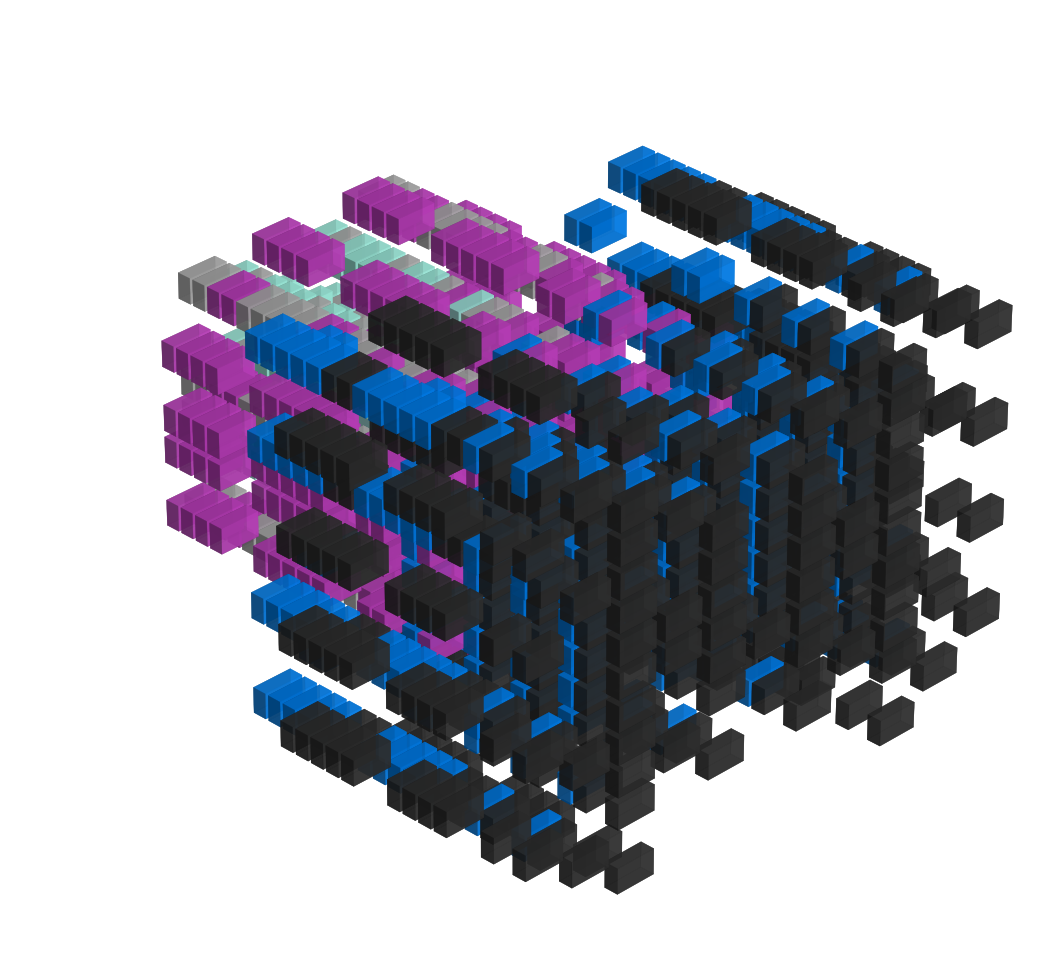
\includegraphics[width=7cm]{src/presets/pattern5-45.png}%           
  \end{adjustbox}                                                        
\caption{Evolution of Preset 5.}                                           
\end{figure}                                                               
\end{minipage}
\hspace{0.1cm}
\begin{minipage}[b]{0.48\linewidth}                                       
                                                                           
\begin{lstlisting}[basicstyle=\ttfamily\scriptsize,caption=Data structure for Preset 5.]
preset5
  .BYTE $00 ; unusedPresetByte
  .BYTE $0C ; smoothingDelay
  .BYTE $02 ; cursorSpeed
  .BYTE $2B ; bufferLength
  .BYTE $01 ; pulseSpeed
  .BYTE $07 ; indexForColorBarDisplay
  .BYTE $07 ; lineWidth
  .BYTE $0C ; sequencerSpeed
  .BYTE $01 ; pulseWidth
  .BYTE $07 ; baseLevel
  ; presetColorValuesArray: 
  .BYTE BLACK,GRAY1,BLUE,GRAY2,PURPLE,GRAY3,CYAN,WHITE
  .BYTE $00 ; trackingActivated
  .BYTE $00 ; lineModeActivated
  .BYTE $06 ; presetIndex
  .BYTE $06 ; currentPatternElement
  .BYTE $03 ; currentSymmetrySetting
\end{lstlisting}
\end{minipage}

\vspace*{-0.7cm}
\begin{minipage}[b]{0.48\linewidth}


                                                                 
\begin{figure}[H]                                                          
  \centering                                                             
  \begin{adjustbox}{width=7cm,center}                                   
  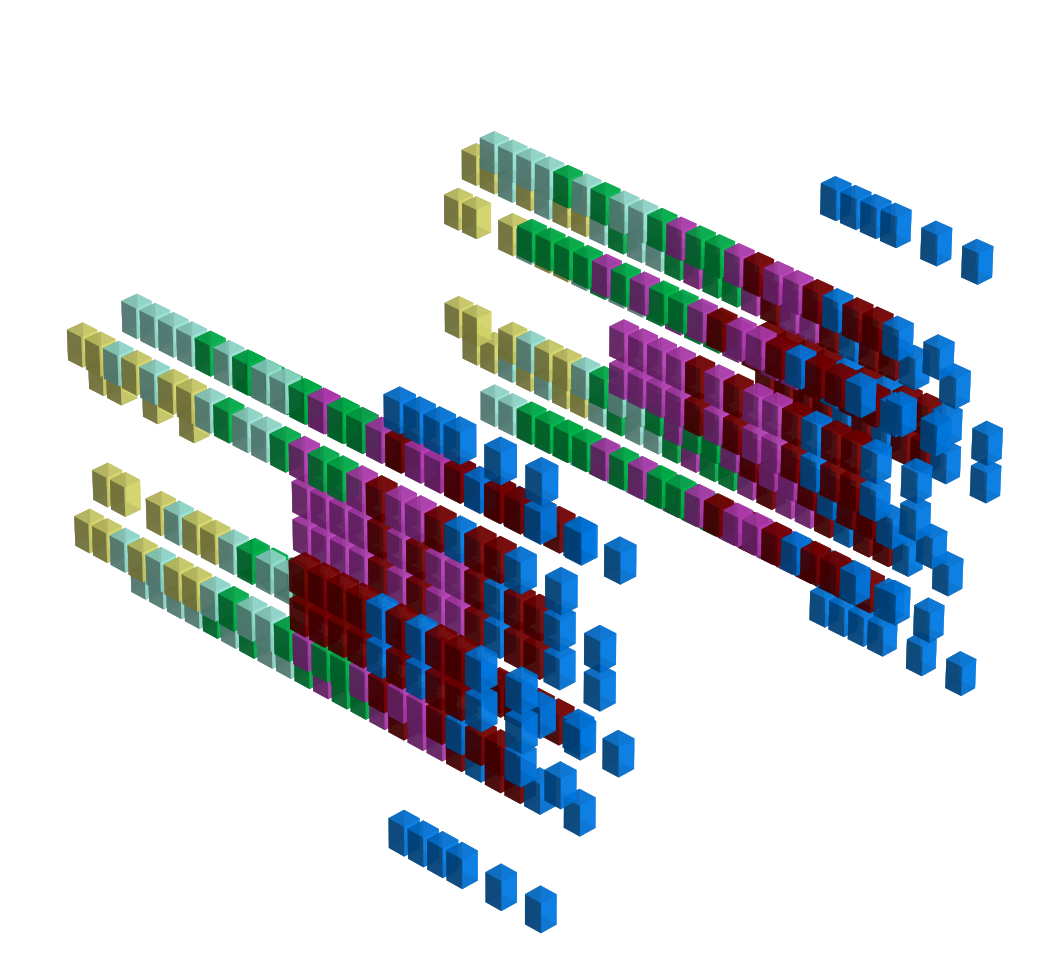
\includegraphics[width=7cm]{src/presets/pattern6-45.png}%           
  \end{adjustbox}                                                        
\caption{Evolution of Preset 6.}                                           
\end{figure}                                                               
                                                                 
                                                                           
\end{minipage}
\hspace{0.1cm}
\begin{minipage}[b]{0.48\linewidth}                                       
\begin{lstlisting}[basicstyle=\ttfamily\scriptsize,caption=Data structure for Preset 6.]
preset6
  .BYTE $00 ; unusedPresetByte
  .BYTE $0F ; smoothingDelay
  .BYTE $02 ; cursorSpeed
  .BYTE $3F ; bufferLength
  .BYTE $01 ; pulseSpeed
  .BYTE $01 ; indexForColorBarDisplay
  .BYTE $07 ; lineWidth
  .BYTE $0F ; sequencerSpeed
  .BYTE $01 ; pulseWidth
  .BYTE $07 ; baseLevel
  ; presetColorValuesArray: 
  .BYTE BLACK,BLUE,RED,PURPLE,GREEN,CYAN,YELLOW,WHITE
  .BYTE $FF ; trackingActivated
  .BYTE $00 ; lineModeActivated
  .BYTE $03 ; presetIndex
  .BYTE $03 ; currentPatternElement
  .BYTE $04 ; currentSymmetrySetting
\end{lstlisting}
\end{minipage}

\clearpage
\begin{minipage}[b]{0.48\linewidth}


                                                                 
\begin{figure}[H]                                                          
  \centering                                                             
  \begin{adjustbox}{width=7cm,center}                                   
  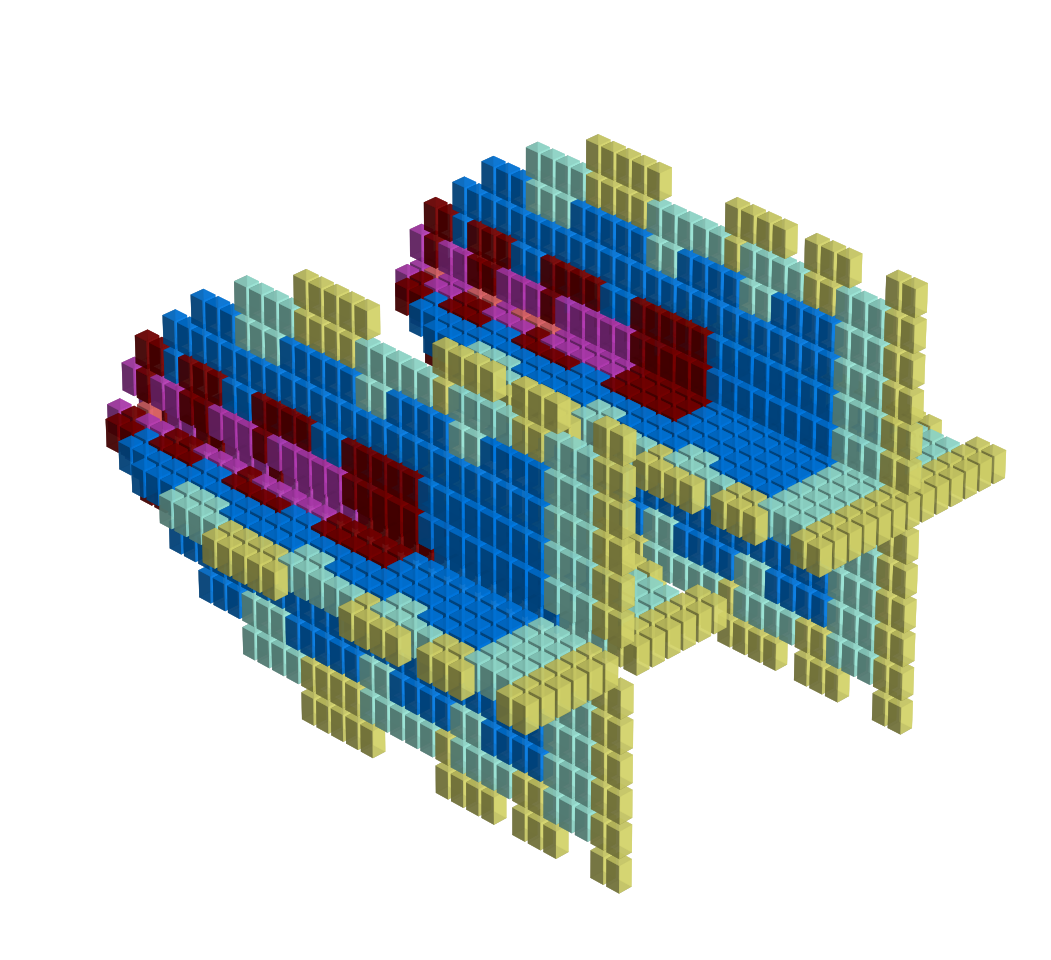
\includegraphics[width=7cm]{src/presets/pattern7-45.png}%           
  \end{adjustbox}                                                        
\caption{Evolution of Preset 7.}                                           
\end{figure}                                                               
                                                                 
                                                                           
\end{minipage}
\hspace{0.1cm}
\begin{minipage}[b]{0.48\linewidth}                                       
\begin{lstlisting}[basicstyle=\ttfamily\scriptsize,caption=Data structure for Preset 7.]
preset7
  .BYTE $00 ; unusedPresetByte
  .BYTE $0B ; smoothingDelay
  .BYTE $01 ; cursorSpeed
  .BYTE $1C ; bufferLength
  .BYTE $02 ; pulseSpeed
  .BYTE $0A ; indexForColorBarDisplay
  .BYTE $07 ; lineWidth
  .BYTE $09 ; sequencerSpeed
  .BYTE $01 ; pulseWidth
  .BYTE $07 ; baseLevel
  ; presetColorValuesArray: 
  .BYTE BLACK,YELLOW,CYAN,LTBLUE,BLUE,RED,PURPLE,LTRED
  .BYTE $00 ; trackingActivated
  .BYTE $00 ; lineModeActivated
  .BYTE $07 ; presetIndex
  .BYTE $07 ; currentPatternElement
  .BYTE $01 ; currentSymmetrySetting
\end{lstlisting}
\end{minipage}

\begin{minipage}[b]{0.48\linewidth}
\begin{figure}[H]                                                          
  \centering                                                             
  \begin{adjustbox}{width=7cm,center}                                   
  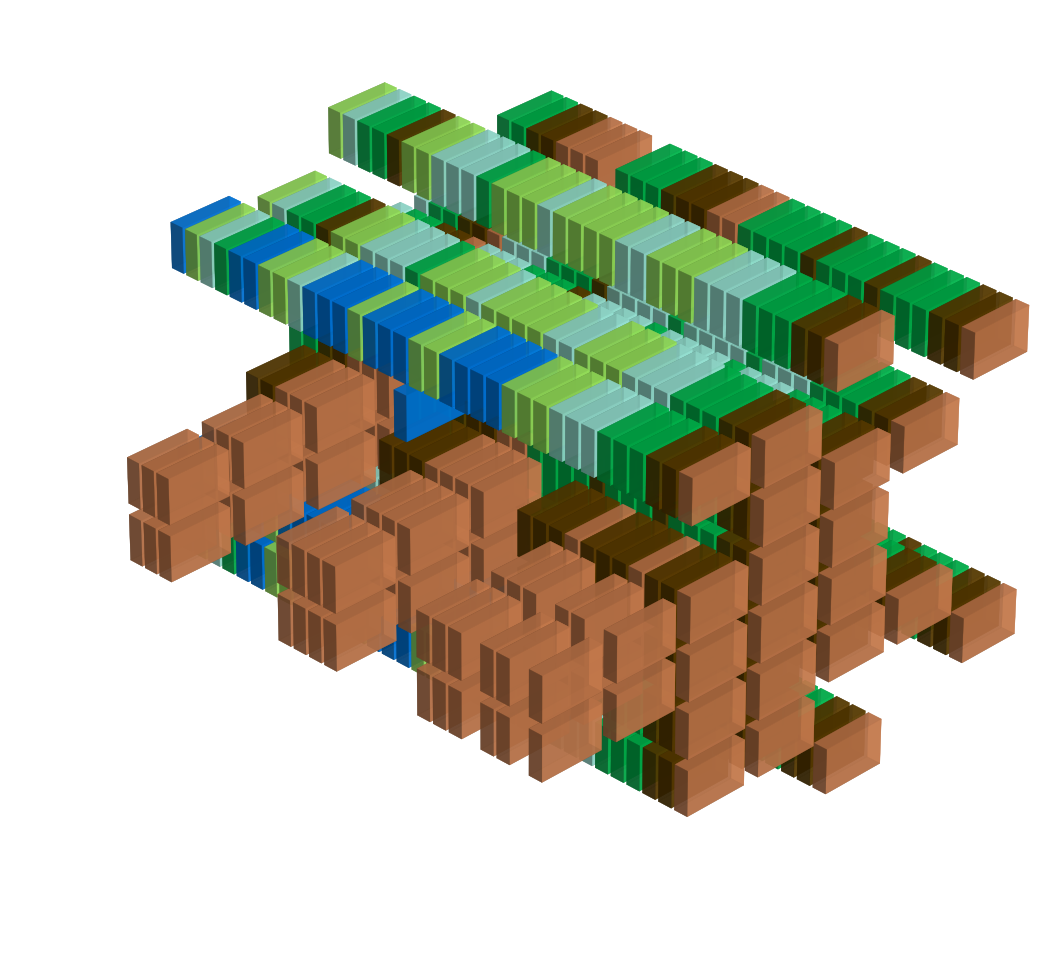
\includegraphics[width=7cm]{src/presets/pattern8-45.png}%           
  \end{adjustbox}                                                        
\caption{Evolution of Preset 8.}                                           
\end{figure}                                                               
                                                                 
                                                                           
\end{minipage}
\hspace{0.1cm}
\begin{minipage}[b]{0.48\linewidth}                                       
\begin{lstlisting}[basicstyle=\ttfamily\scriptsize,caption=Data structure for Preset 8.]
preset8
  .BYTE $00 ; unusedPresetByte
  .BYTE $04 ; smoothingDelay
  .BYTE $01 ; cursorSpeed
  .BYTE $28 ; bufferLength
  .BYTE $02 ; pulseSpeed
  .BYTE $01 ; indexForColorBarDisplay
  .BYTE $07 ; lineWidth
  .BYTE $0A ; sequencerSpeed
  .BYTE $01 ; pulseWidth
  .BYTE $07 ; baseLevel
  ; presetColorValuesArray: 
  .BYTE BLACK,ORANGE,BROWN,GREEN,CYAN,LTGREEN,LTBLUE,BLUE
  .BYTE $FF ; trackingActivated
  .BYTE $00 ; lineModeActivated
  .BYTE $01 ; presetIndex
  .BYTE $01 ; currentPatternElement
  .BYTE $03 ; currentSymmetrySetting
\end{lstlisting}
\end{minipage}


\clearpage
\textbf{Lines 1189-1231. \icode{\textbf{DisplayPresetMessage}}} 
\begin{lstlisting}
;-------------------------------------------------------
; DisplayPresetMessage
;-------------------------------------------------------
DisplayPresetMessage    
        LDA shiftPressed
        AND #$04
        BEQ WriteTemplateTextForPreset

        JMP EditCustomPattern

WriteTemplateTextForPreset
        TXA 
        PHA 
        JSR ClearLastLineOfScreen

        LDX #$00
_Loop   LDA txtPreset,X
        STA statusFieldName,X
        INX 
        CPX #$10
        BNE _Loop

PrepareToWritePresetValue
        PLA 
        PHA 
        TAX 
        BEQ FinishedUpdatingDisplay

WriteTemplateTextForPresetDigits   
        INC presetDigitOne
        LDA presetDigitOne
        CMP #"0"
        BNE GoToNext
        LDA #"0"
        STA presetDigitOne
        INC presetDigitTwo
GoToNext   
        DEX 
        BNE WriteTemplateTextForPresetDigits

FinishedUpdatingDisplay   
        JMP UpdateCurrentActivePreset

WriteLastLineBufferAndReturn    
        JSR WriteLastLineBufferToScreen
        RTS 
\end{lstlisting}
\clearpage

\textbf{Lines 1189-1231. \icode{\textbf{DisplayPresetMessage}}:} Our objective here is modest enough. Display something like the following
on the bottom of the screen to show the player the preset they've selected:
\begin{figure}[H]                                                          
  \centering                                                             
  \frame{
\includegraphics[width=7cm]{src/presets/activated.png}}%
\caption{Our desired result!}
\end{figure}                                                               
\vspace*{-0.7cm}
Our data for this is stored as follows:
\begin{lstlisting}
txtPreset
        .TEXT 'PRESET 00       :'
txtPresetActivatedStored
        .TEXT 'ACTIVATED        '
        .TEXT 'DATA STORED      '
\end{lstlisting}
\icode{txtPreset} contains the template for displaying the selected value. \icode{txtPresetActivatedStored} contains two templates: one for
when we're activating a selected preset and the second for when we're storing currently configured values as a preset.

\textbf{Lines 1189-1231. \icode{\textbf{WriteTemplateTextForPreset}}:} We'll split the task in two. First let's get some of the boiler plate text
above ('PRESET 00         :') set up. This is what we do in here. (We'll deal with writing 'ACTIVATED' a little later.) With the help of a little
loop the contents of \icode{txtPreset} get stored in \icode{statusFieldName}.

\textbf{Lines 1189-1231. \icode{\textbf{WriteTemplateTextForPresetDigits}}:} Now we write the corresponding value for the selected preset. Remeber that
\icode{X} contains the selected value, so we increment the displayed value in a loop while simultaneously decrementing the value in \icode{X}. Once
\icode{X} reaches zero the displayed value will match the selected value.

\textbf{Lines 1189-1231. \icode{\textbf{FinishedUpdatingDisplay}}:} When we've finished we'll now have something like this displayed on the screen.
\begin{figure}[H]                                                          
  \centering                                                             
  \frame{
\includegraphics[width=7cm]{src/presets/activated-part.png}}%
\caption{Making progress!}
\end{figure}                                                               
\vspace*{-0.7cm}

We're ready to fill out the 'ACTIVATED' part and actually load the preset values. So let's \icode{JMP} to \icode{UpdateCurrentActivePreset} and do that!

\clearpage
\begin{minipage}[b]{0.48\linewidth}
\begin{figure}[H]                                                          
  \centering                                                             
  \begin{adjustbox}{width=7cm,center}                                   
  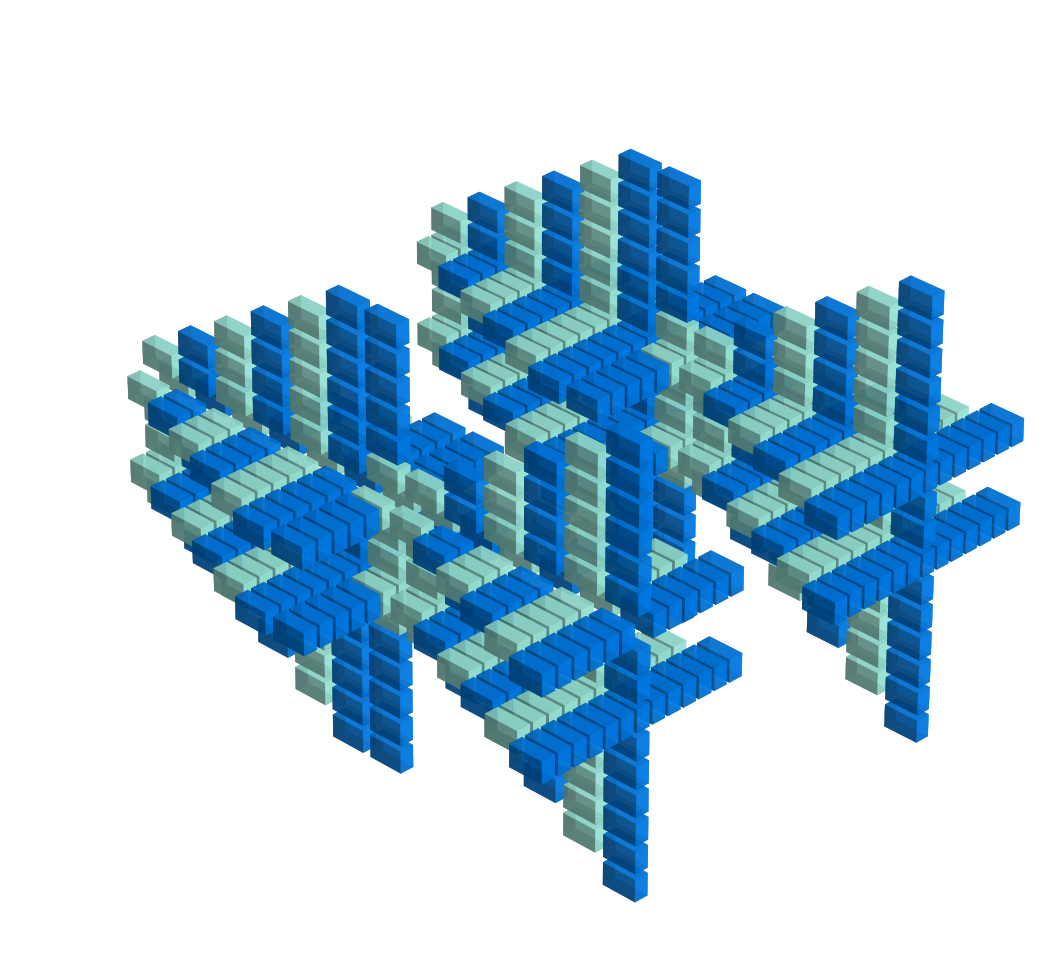
\includegraphics[width=7cm]{src/presets/pattern9-45.png}%           
  \end{adjustbox}                                                        
\caption{Evolution of Preset 9.}                                           
\end{figure}                                                               
\end{minipage}
\hspace{0.1cm}
\begin{minipage}[b]{0.48\linewidth}                                       
\begin{lstlisting}[basicstyle=\ttfamily\scriptsize,caption=Data structure for Preset 9.]
preset9
  .BYTE $00 ; unusedPresetByte
  .BYTE $11 ; smoothingDelay
  .BYTE $01 ; cursorSpeed
  .BYTE $0D ; bufferLength
  .BYTE $07 ; pulseSpeed
  .BYTE $01 ; indexForColorBarDisplay
  .BYTE $07 ; lineWidth
  .BYTE $0C ; sequencerSpeed
  .BYTE $01 ; pulseWidth
  .BYTE $07 ; baseLevel
  ; presetColorValuesArray: 
  .BYTE BLACK,BLUE,CYAN,BLUE,CYAN,BLUE,CYAN,BLUE
  .BYTE $FF ; trackingActivated
  .BYTE $00 ; lineModeActivated
  .BYTE $07 ; presetIndex
  .BYTE $07 ; currentPatternElement
  .BYTE $04 ; currentSymmetrySetting
\end{lstlisting}
\end{minipage}

\vspace*{-0.7cm}
\begin{minipage}[b]{0.48\linewidth}


                                                                 
\begin{figure}[H]                                                          
  \centering                                                             
  \begin{adjustbox}{width=7cm,center}                                   
  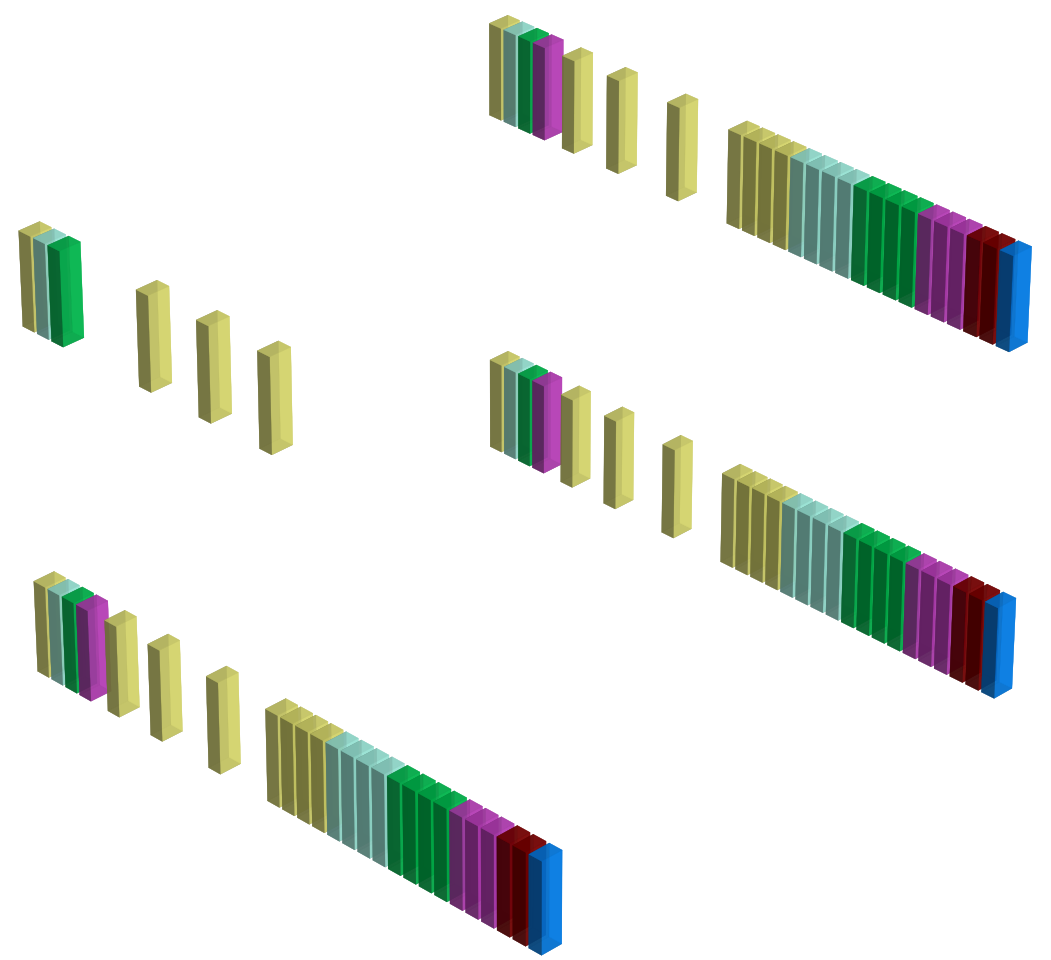
\includegraphics[width=7cm]{src/presets/pattern10-45.png}%           
  \end{adjustbox}                                                        
\caption{Evolution of Preset 10.}                                           
\end{figure}                                                               
                                                                 
                                                                           
\end{minipage}
\hspace{0.1cm}
\begin{minipage}[b]{0.48\linewidth}                                       
\begin{lstlisting}[basicstyle=\ttfamily\scriptsize,caption=Data structure for Preset 10.]
preset10
  .BYTE $00 ; unusedPresetByte
  .BYTE $01 ; smoothingDelay
  .BYTE $02 ; cursorSpeed
  .BYTE $1F ; bufferLength
  .BYTE $02 ; pulseSpeed
  .BYTE $09 ; indexForColorBarDisplay
  .BYTE $04 ; lineWidth
  .BYTE $08 ; sequencerSpeed
  .BYTE $01 ; pulseWidth
  .BYTE $07 ; baseLevel
  ; presetColorValuesArray: 
  .BYTE BLACK,BLUE,RED,RED,PURPLE,LTRED,ORANGE,BROWN
  .BYTE $FF ; trackingActivated
  .BYTE $01 ; lineModeActivated
  .BYTE $00 ; presetIndex
  .BYTE $00 ; currentPatternElement
  .BYTE $04 ; currentSymmetrySetting
\end{lstlisting}
\end{minipage}

\clearpage
\begin{minipage}[b]{0.48\linewidth}
\begin{figure}[H]                                                          
  \centering                                                             
  \begin{adjustbox}{width=7cm,center}                                   
  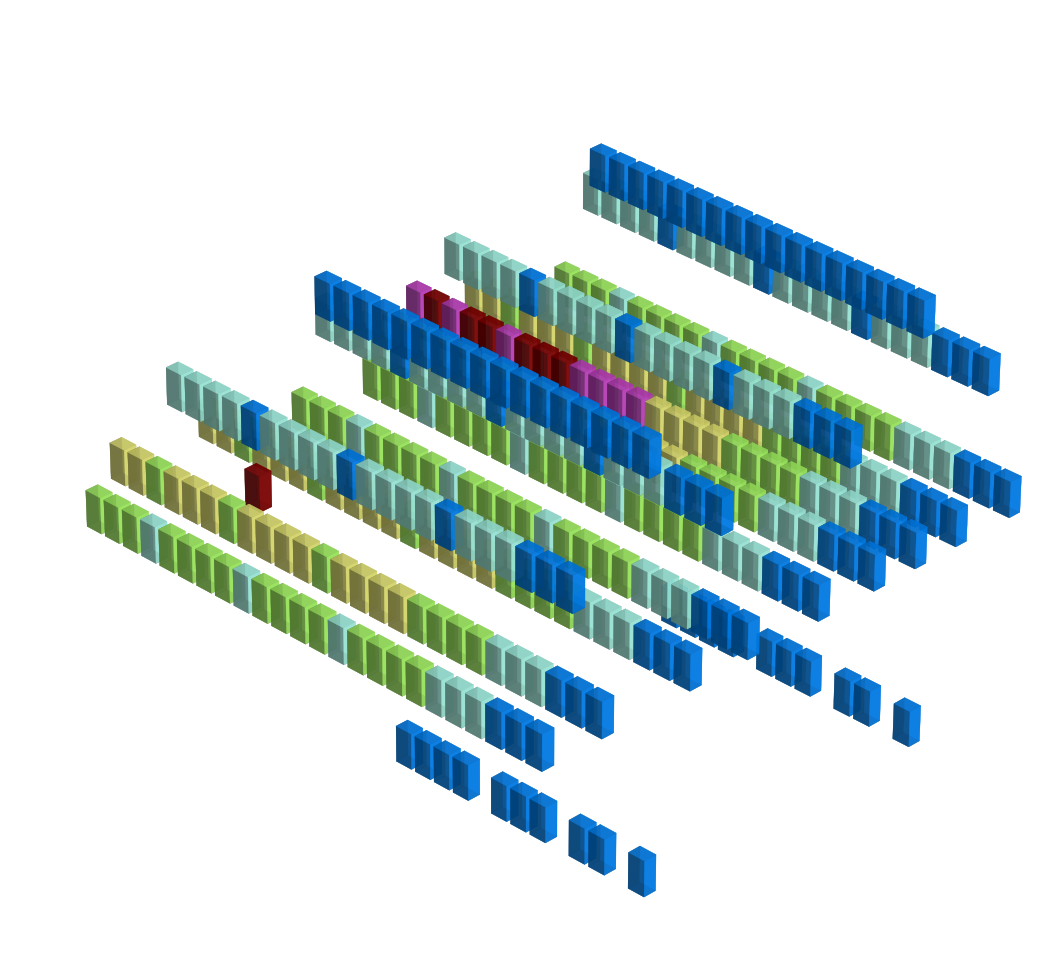
\includegraphics[width=7cm]{src/presets/pattern11-45.png}%           
  \end{adjustbox}                                                        
\caption{Evolution of Preset 11.}                                           
\end{figure}                                                               
                                                                 
                                                                           
\end{minipage}
\hspace{0.1cm}
\begin{minipage}[b]{0.48\linewidth}                                       
\begin{lstlisting}[basicstyle=\ttfamily\scriptsize,caption=Data structure for Preset 11.]
preset11
  .BYTE $00 ; unusedPresetByte
  .BYTE $01 ; smoothingDelay
  .BYTE $01 ; cursorSpeed
  .BYTE $13 ; bufferLength
  .BYTE $06 ; pulseSpeed
  .BYTE $01 ; indexForColorBarDisplay
  .BYTE $07 ; lineWidth
  .BYTE $08 ; sequencerSpeed
  .BYTE $05 ; pulseWidth
  .BYTE $07 ; baseLevel
  ; presetColorValuesArray: 
  .BYTE BLACK,BLUE,RED,PURPLE,GREEN,CYAN,YELLOW,WHITE
  .BYTE $FF ; trackingActivated
  .BYTE $00 ; lineModeActivated
  .BYTE $0F ; presetIndex
  .BYTE $0F ; currentPatternElement
  .BYTE $04 ; currentSymmetrySetting
\end{lstlisting}
\end{minipage}

\vspace*{-0.7cm}
\begin{minipage}[b]{0.48\linewidth}


                                                                 
\begin{figure}[H]                                                          
  \centering                                                             
  \begin{adjustbox}{width=7cm,center}                                   
  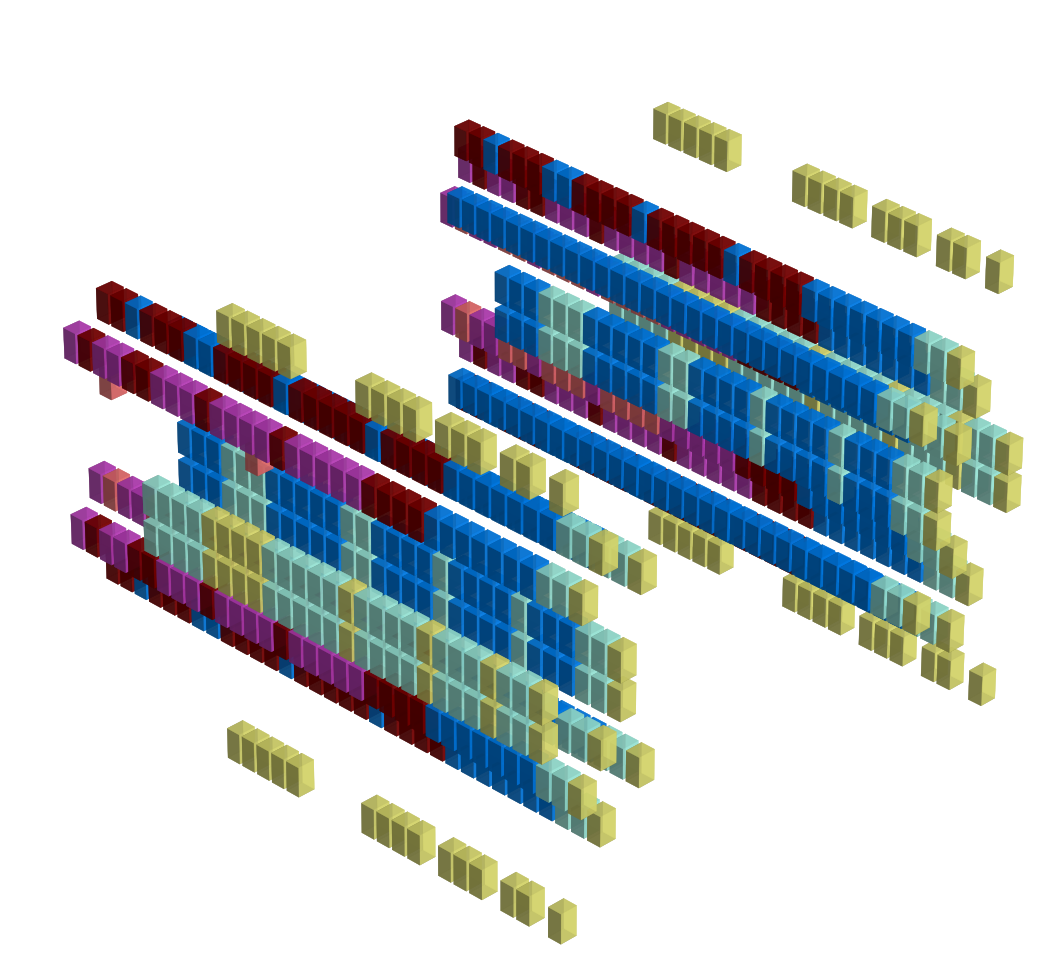
\includegraphics[width=7cm]{src/presets/pattern12-45.png}%           
  \end{adjustbox}                                                        
\caption{Evolution of Preset 12.}                                           
\end{figure}                                                               
                                                                 
                                                                           
\end{minipage}
\hspace{0.1cm}
\begin{minipage}[b]{0.48\linewidth}                                       
\begin{lstlisting}[basicstyle=\ttfamily\scriptsize,caption=Data structure for Preset 12.]
preset12
  .BYTE $00 ; unusedPresetByte
  .BYTE $0C ; smoothingDelay
  .BYTE $02 ; cursorSpeed
  .BYTE $28 ; bufferLength
  .BYTE $01 ; pulseSpeed
  .BYTE $02 ; indexForColorBarDisplay
  .BYTE $07 ; lineWidth
  .BYTE $09 ; sequencerSpeed
  .BYTE $01 ; pulseWidth
  .BYTE $07 ; baseLevel
  ; presetColorValuesArray: 
  .BYTE BLACK,BLUE,LTBLUE,CYAN,LTGREEN,YELLOW,PURPLE,RED
  .BYTE $00 ; trackingActivated
  .BYTE $00 ; lineModeActivated
  .BYTE $0A ; presetIndex
  .BYTE $0A ; currentPatternElement
  .BYTE $01 ; currentSymmetrySetting
\end{lstlisting}
\end{minipage}

\clearpage
\textbf{Lines 1189-1231. \icode{\textbf{UpdateCurrentActivePreset}}} 
\begin{lstlisting}
;-------------------------------------------------------
; UpdateCurrentActivePreset
;-------------------------------------------------------
UpdateCurrentActivePreset    
        LDA shiftPressed
        AND #SHIFT_PRESSED
        ASL 
        ASL 
        ASL 
        ASL 
        TAY 

DisplayActivatedOrStored
        LDX #$00
_Loop   LDA txtPresetActivatedStored,Y
        STA customPatternValueBufferMessage,X
        INY 
        INX 
        CPX #DISPLAY_LINE_LENGTH
        BNE _Loop

        LDA shiftPressed
        AND #SHIFT_PRESSED
        BNE StoreCurrentValuesAsPreset

        ; Shift wasn't pressed, so load the selected preset.
        JMP RefreshPresetData

StoreCurrentValuesAsPreset   
        PLA 
        TAX 
        JSR GetPresetPointersUsingXRegister

        LDY #$00
        LDX #$00
_Loop   LDA presetValueArray,X
        STA (presetSequenceDataLoPtr),Y
        INY 
        INX 
        CPX #$15
        BNE _Loop

        LDA currentPatternElement
        STA (presetSequenceDataLoPtr),Y
        INY 
        LDA currentSymmetrySetting
        STA (presetSequenceDataLoPtr),Y
        JMP WriteLastLineBufferAndReturn
\end{lstlisting}
\clearpage

\textbf{Lines 1189-1231. \icode{\textbf{UpdateCurrentActivePreset}}:} In the current path we're following (the one where we load a selected preset)
we only have to concern ourselves with the first half of the routine opposite. This is because the second half is the part that looks after storing
currently configured values to a preset, as opposed to loading one.

So the only part that we execute here is \icode{DisplayActivatedOrStored} which finishes off our status text with the 'ACTIVATED' string. Now we loop
through our text in \icode{txtPresetActivatedStored}:
\begin{lstlisting}
txtPresetActivatedStored
        .TEXT ' ACTIVATED       '
\end{lstlisting}
and write it to storage starting at \icode{customPatternValueBufferMessage}. 

This is the final piece in \icode{statusLineBuffer} that we need to fill out
in order to display our text. We've already filled out the first two parts of this data structure (\icode{statusFieldName} and \icode{presetDigitOne/presetDigitTwo} 
and now have it in the state below: 

\begin{lstlisting}
statusLineBuffer
statusFieldName                 .TEXT 'PRESET '
presetDigitOne                  .TEXT '0'
presetDigitTwo                  .TEXT '2'
presetDigitThree                .TEXT ' '
customPatternValueBufferPtr     .TEXT '   '
customPatternValueBufferMessage .TEXT 'ACTIVATED     '
\end{lstlisting}

Later on we will actually write this buffer to the screen by copying all the values in \icode{statusLineBuffer} together to the last line on the screen:

\begin{lstlisting}
WriteLastLineBufferToScreen    
        LDX #NUM_COLS
_Loop   
        LDA statusLineBuffer - $01,X
        AND #$3F
        STA SCREEN_RAM + $03BF,X
        LDA #$0C
        STA COLOR_RAM + $03BF,X
        DEX 
        BNE _Loop
        RTS 
\end{lstlisting}

For now though we still have to actually load the preset data. So we \icode{JMP} to \icode{RefreshPresetData} after we've finished looping through \icode{DisplayActivatedOrStored}.

\clearpage
\vspace*{-0.5cm}
\begin{minipage}[b]{0.48\linewidth}


                                                                 
\begin{figure}[H]                                                          
  \centering                                                             
  \begin{adjustbox}{width=7cm,center}                                   
  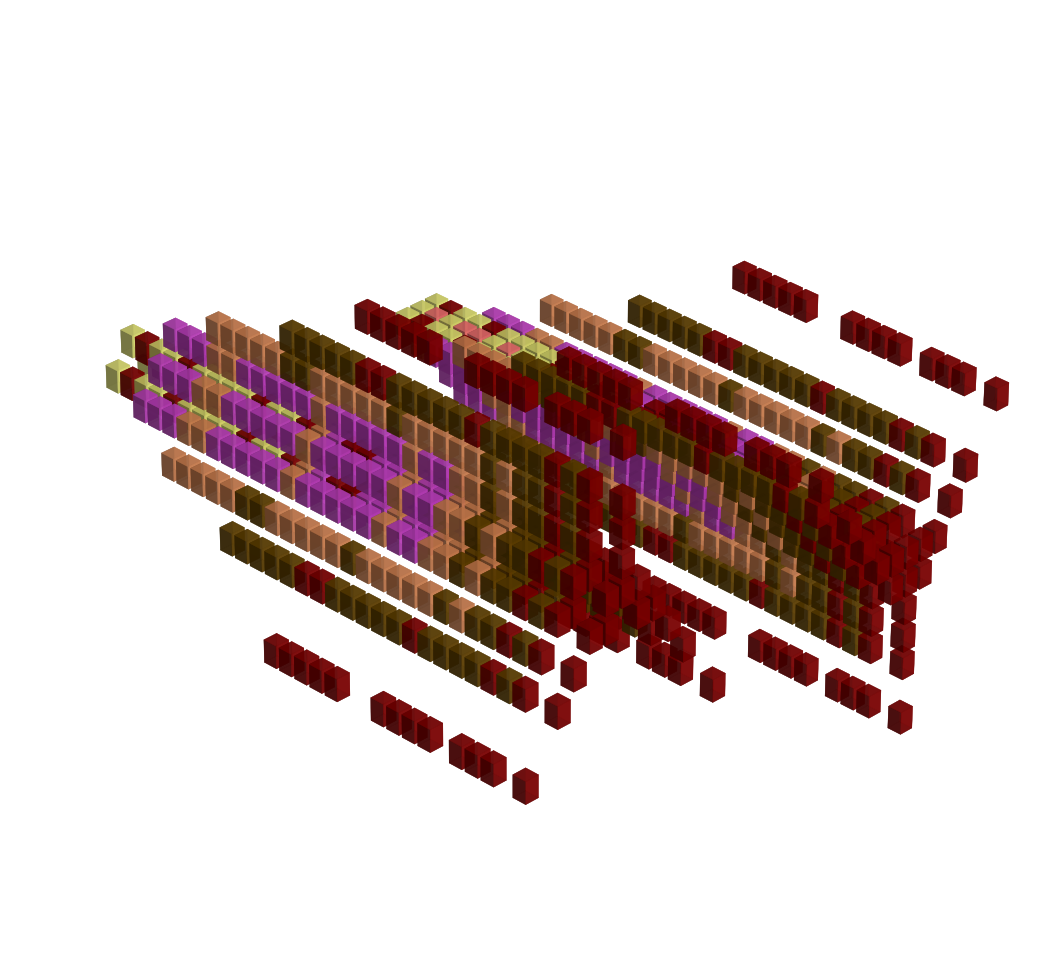
\includegraphics[width=7cm]{src/presets/pattern13-45.png}%           
  \end{adjustbox}                                                        
\caption{Evolution of Preset 13.}                                           
\end{figure}                                                               
                                                                 
                                                                           
\end{minipage}
\hspace{0.1cm}
\begin{minipage}[b]{0.48\linewidth}                                       
\begin{lstlisting}[basicstyle=\ttfamily\scriptsize,caption=Data structure for Preset 13.]
preset13
  .BYTE $00 ; unusedPresetByte
  .BYTE $0B ; smoothingDelay
  .BYTE $01 ; cursorSpeed
  .BYTE $1C ; bufferLength
  .BYTE $02 ; pulseSpeed
  .BYTE $0A ; indexForColorBarDisplay
  .BYTE $07 ; lineWidth
  .BYTE $09 ; sequencerSpeed
  .BYTE $01 ; pulseWidth
  .BYTE $07 ; baseLevel
  ; presetColorValuesArray: 
  .BYTE BLACK,YELLOW,CYAN,LTBLUE,BLUE,RED,PURPLE,LTRED
  .BYTE $00 ; trackingActivated
  .BYTE $00 ; lineModeActivated
  .BYTE $03 ; presetIndex
  .BYTE $03 ; currentPatternElement
  .BYTE $04 ; currentSymmetrySetting
\end{lstlisting}
\end{minipage}

\begin{minipage}[b]{0.48\linewidth}


                                                                 
\begin{figure}[H]                                                          
  \centering                                                             
  \begin{adjustbox}{width=7cm,center}                                   
  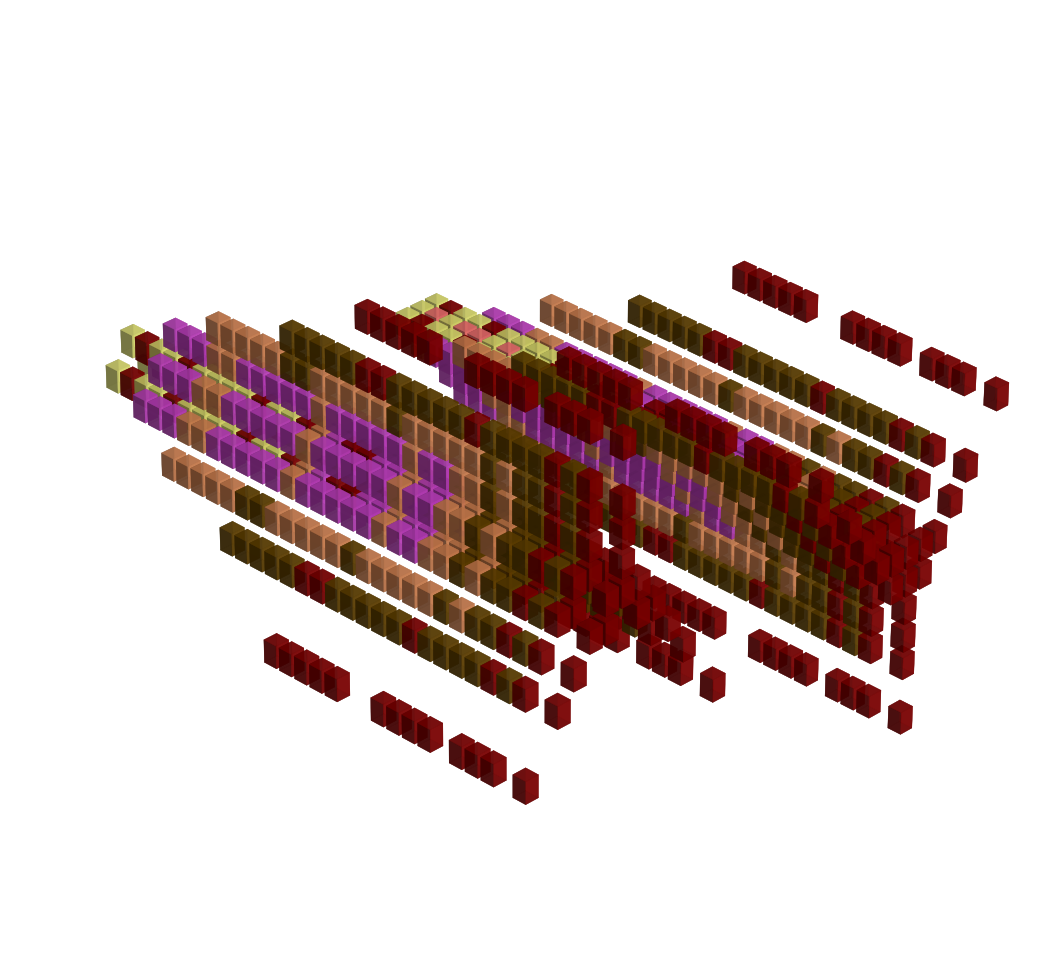
\includegraphics[width=7cm]{src/presets/pattern14-45.png}%           
  \end{adjustbox}                                                        
\caption{Evolution of Preset 14.}                                           
\end{figure}                                                               
                                                                 
                                                                           
\end{minipage}
\hspace{0.1cm}
\begin{minipage}[b]{0.48\linewidth}                                       
\begin{lstlisting}[basicstyle=\ttfamily\scriptsize,caption=Data structure for Preset 14.]
preset14
  .BYTE $00 ; unusedPresetByte
  .BYTE $0C ; smoothingDelay
  .BYTE $02 ; cursorSpeed
  .BYTE $2B ; bufferLength
  .BYTE $01 ; pulseSpeed
  .BYTE $0A ; indexForColorBarDisplay
  .BYTE $07 ; lineWidth
  .BYTE $08 ; sequencerSpeed
  .BYTE $01 ; pulseWidth
  .BYTE $07 ; baseLevel
  ; presetColorValuesArray: 
  .BYTE BLACK,RED,BROWN,ORANGE,PURPLE,RED,YELLOW,LTRED
  .BYTE $FF ; trackingActivated
  .BYTE $00 ; lineModeActivated
  .BYTE $04 ; presetIndex
  .BYTE $04 ; currentPatternElement
  .BYTE $02 ; currentSymmetrySetting
\end{lstlisting}
\end{minipage}

\clearpage
\begin{minipage}[b]{0.48\linewidth}
\begin{figure}[H]                                                          
  \centering                                                             
  \begin{adjustbox}{width=7cm,center}                                   
  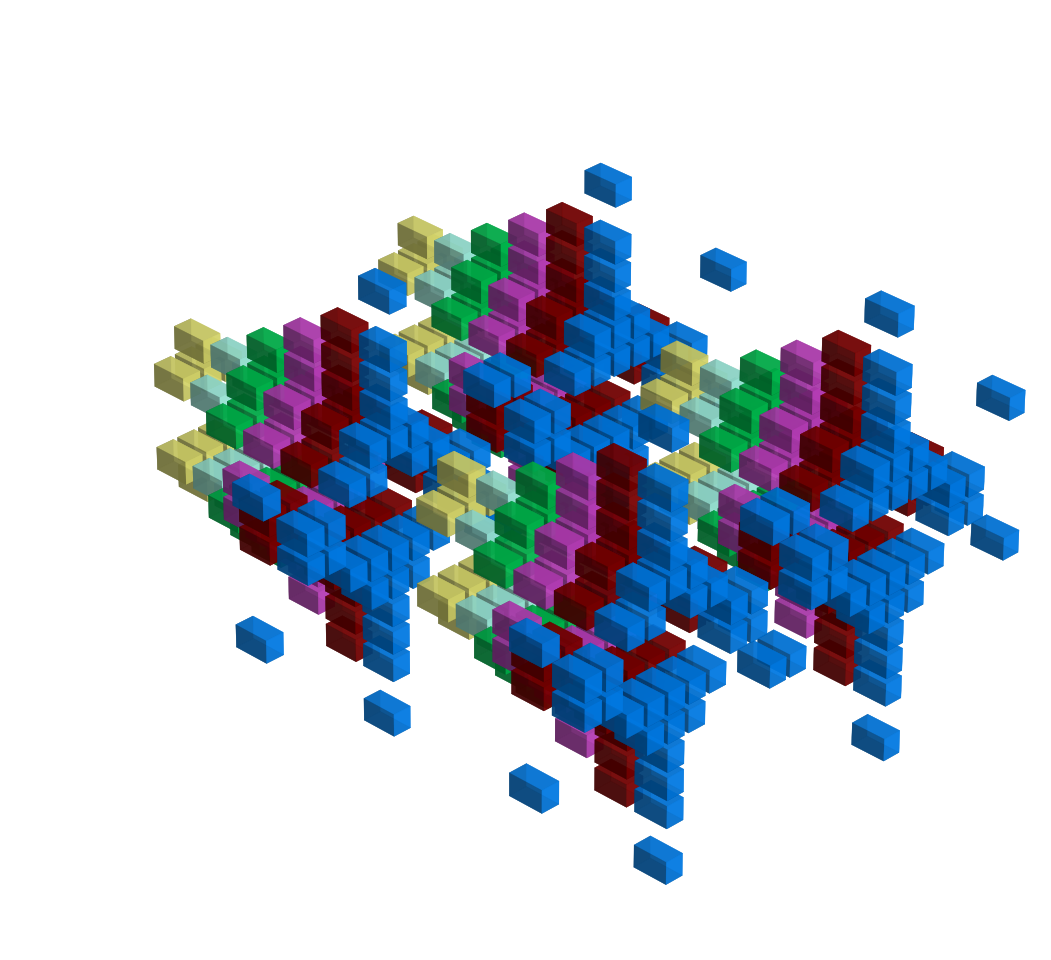
\includegraphics[width=7cm]{src/presets/pattern15-45.png}%           
  \end{adjustbox}                                                        
\caption{Evolution of Preset 15.}                                           
\end{figure}                                                               
                                                                 
                                                                           
\end{minipage}
\hspace{0.1cm}
\begin{minipage}[b]{0.48\linewidth}                                       
\begin{lstlisting}[basicstyle=\ttfamily\scriptsize,caption=Data structure for Preset 15.]
preset15
  .BYTE $00 ; unusedPresetByte
  .BYTE $03 ; smoothingDelay
  .BYTE $01 ; cursorSpeed
  .BYTE $1F ; bufferLength
  .BYTE $06 ; pulseSpeed
  .BYTE $01 ; indexForColorBarDisplay
  .BYTE $07 ; lineWidth
  .BYTE $00 ; sequencerSpeed
  .BYTE $01 ; pulseWidth
  .BYTE $07 ; baseLevel
  ; presetColorValuesArray: 
  .BYTE BLACK,BLUE,RED,PURPLE,GREEN,CYAN,YELLOW,WHITE
  .BYTE $FF ; trackingActivated
  .BYTE $00 ; lineModeActivated
  .BYTE $04 ; presetIndex
  .BYTE $04 ; currentPatternElement
  .BYTE $04 ; currentSymmetrySetting
\end{lstlisting}
\end{minipage}


\clearpage
\textbf{Lines 1189-1231. \icode{\textbf{RefreshPresetData}}} 
\begin{lstlisting}
RefreshPresetData    
        PLA 
        TAX 
        JSR GetPresetPointersUsingXRegister

        LDY #BUFFER_LENGTH
        LDA (presetSequenceDataLoPtr),Y
        CMP bufferLength
        BEQ CheckColorValuesForDifferences

        JSR ResetCurrentActiveMode
        JMP LoadSelectedPresetSequence
        ; Returns

        ; Check the preset against current data
        ; and reload if different.
CheckColorValuesForDifferences   
        LDX #$00
        LDY #$07
_Loop   LDA (presetSequenceDataLoPtr),Y
        CMP presetColorValuesArray,X
        BNE LoadSelectedPresetSequence
        INY 
        INX 
        CPX #$08
        BNE _Loop

        JMP LoadSelectedPresetSequence

\end{lstlisting}
\clearpage


\textbf{Lines 1189-1231. \icode{\textbf{RefreshPresetData}}:} Our first order of business here is to get the location of the selected preset
in our storage. This is where storing the value of the of selected preset in \icode{X} will come in useful. 

We call \icode{GetPresetPointersUsingXRegister} to get this done. We've encountered this design pattern 
previously: we use the value in X to iterate from the start of the preset data (given by \icode{presetSequenceData} and stored in a pair of pointers
(\icode{presetSequenceData\-LoPtr/preset\-SequenceDataHiPtr}. We then iterate from zero until we reach the value of the preset selected by the player, 
incrementing \icode{presetSequenceDataLoPtr} by 32 bytes each time. Once we reach the value selected, our two pointers will contain the address
of the selected preset data. In the case of preset '2' this means we will start at \icode{\$C000} and end up at \icode{\$C040}.
\begin{lstlisting}
GetPresetPointersUsingXRegister   
        LDA #>presetSequenceData
        STA presetSequenceDataHiPtr
        LDA #<presetSequenceData
        STA presetSequenceDataLoPtr
        TXA 
        BEQ ReturnFromPointers

_Loop   LDA presetSequenceDataLoPtr
        CLC 
        ADC #$20
        STA presetSequenceDataLoPtr
        LDA presetSequenceDataHiPtr
        ADC #$00
        STA presetSequenceDataHiPtr
        DEX 
        BNE _Loop

ReturnFromPointers   
        RTS 
\end{lstlisting}

For some reason not clear to me, the rest of this routine goes to a bit of trouble in checking the data we're about to load and whether it's the same
as the preset data we already have loaded. All of these checks end in the same outcome: we call \icode{LoadSelectedPresetSequence} to actually load 
the data anyway. So, to me at least, it looks like there was the intention to optimize in some way here but it was abandoned. Despite all of the footling
around we just go ahead and load the preset data.

\clearpage

\textbf{Lines 1189-1231. \icode{\textbf{LoadSelectedPresetSequence}}} 
\begin{lstlisting}
LoadSelectedPresetSequence    
        LDA #$FF
        STA currentModeActive

        ; Copy the value from the preset sequence into 
        ; current storage.
        LDY #0
_Loop   LDA (presetSequenceDataLoPtr),Y
        STA presetValueArray,Y
        INY 
        CPY #$15
        BNE _Loop

        LDA (presetSequenceDataLoPtr),Y
        STA currentPatternElement

        INY 
        LDA (presetSequenceDataLoPtr),Y
        STA currentSymmetrySetting

        JMP WriteLastLineBufferAndReturn
\end{lstlisting}
\clearpage
\textbf{Lines 1189-1231. \icode{\textbf{LoadSelectedPresetSequence}}:} After all this trouble we go ahead and load the data using our pointers into 
\icode{presetValueArray}. As we saw at the start of the chapter the fact that our preset values are stored contiguously means that a simple loop
will do the bulk of the job. However there are two trailing items the \icode{currentPatternElement} and \icode{currentSymmetrySetting} that we need
to pick out by name. 

When we're done we finally write the status line to the screen and return. That completes loading of the preset data. Now we can take a look at some
of these individual settings more closely.

